\documentclass[handout]{beamer}
%==============================================================
% Common Beamer Preamble for Course Lectures: Training and Scaling Language Models
%==============================================================

\usepackage[utf8]{inputenc}
\usepackage[T1]{fontenc}
\usepackage{hyperref}
\usepackage{amsmath,amssymb,xcolor,multicol,booktabs,colortbl}
\usepackage{graphicx,listings}
\renewcommand{\figurename}{Figure.}
\renewcommand{\tablename}{Table.}

% ---- TikZ Libraries ----
\usepackage{tikz}
\usetikzlibrary{positioning,arrows.meta,shapes.geometric,calc,fit,backgrounds,decorations.pathreplacing}

% ---- Presentation defaults ----
\setbeamertemplate{navigation symbols}{}
\setbeamersize{text margin left=0.55cm,text margin right=0.55cm}
\setbeamerfont{title}{size=\LARGE,series=\bfseries}
\setbeamerfont{subtitle}{size=\large}

% ---- FontAwesome fallback ----
\IfFileExists{fontawesome5.sty}{%
  \usepackage{fontawesome5}%
}{%
  \providecommand{\faMicrochip}{}%
  \providecommand{\faComments}{}%
  \providecommand{\faTools}{}%
  \providecommand{\faCheckCircle}{}%
  \providecommand{\faExclamationTriangle}{}%
  \providecommand{\faImage}{}%
  \providecommand{\faRobot}{}%
  \providecommand{\faTerminal}{}%
  \providecommand{\faBook}{}%
  \providecommand{\faRedo}{}%
  \providecommand{\faLayerGroup}{}%
  \providecommand{\faCogs}{}%
  \providecommand{\faDatabase}{}%
  \providecommand{\faHdd}{}%
  \providecommand{\faNetworkWired}{}%
}

% ---- Theme Style and Semantic Colors ----
%==============================================================
% Centralized Semantic Color Definitions for LLMs Presentation
%==============================================================

% ---- Base Template / Theme Colors (Aligned with Palette B) ----
\definecolor{themenavy}{RGB}{22,70,102}       % Palette B primary cerulean: #164666
\definecolor{themeblue}{RGB}{22,70,102}       % Primary alias
\definecolor{primarylight}{RGB}{34,92,132}    % Primary light: #225c84
\definecolor{themeteal}{RGB}{0,159,176}       % Accent cyan-teal: #009fb0
\colorlet{main_color}{themenavy}
\colorlet{accent}{themeteal}

\definecolor{accentdark}{RGB}{0,108,120}      % Deep cyan-teal for contrast text
\definecolor{accentlight}{RGB}{56,178,214}    % Slate accent cyan: #38b2d6
\definecolor{leafred}{RGB}{197,93,61}         % Terracotta red for branches/leaves

% ---- Website Panel & Border Neutrals ----
\definecolor{panelbg}{RGB}{237,245,249}       % Course-panel: #edf5f9
\definecolor{panelborder}{RGB}{204,226,238}   % Course-border: #cce2ee

% ---- Code listing style (syntax highlights) ----
\definecolor{deepblue}{RGB}{22,70,102}
\definecolor{deepred}{rgb}{0.6,0,0}
\definecolor{deepgreen}{RGB}{0,135,150}
\definecolor{halfgray}{gray}{0.55}

% ---- Semantic Theme Navy / Cerulean Shades ----
\colorlet{themebluebg}{panelbg}               % Panel #edf5f9
\colorlet{themebluecard}{main_color!8}        % Mild card background fills
\colorlet{themeblueborder}{panelborder}       % Border #cce2ee
\colorlet{themebluemid}{themeteal!60}         % Accent mid-contrast
\colorlet{themebluedraw}{main_color!80}       % Strong outline draws/strokes

% ---- Semantic Secondary Accent Teal Shades ----
\colorlet{accentdarkbg}{themeteal!10}        % Light secondary background fills
\colorlet{accentdarkdraw}{themeteal}         % Secondary outlines/strokes/text/axes

% ---- Functional Colors: Success Green ----
\definecolor{successgreen}{RGB}{55,145,55}
\colorlet{successbg}{successgreen!8}
\colorlet{successdraw}{successgreen!75}

% ---- Functional Colors: Alert Red ----
\definecolor{alertred}{RGB}{197,55,55}
\colorlet{alertbg}{alertred!8}
\colorlet{alertdraw}{alertred!75}

% ---- Functional Colors: Warning Orange ----
\definecolor{warningorange}{RGB}{220,110,30}
\colorlet{warningbg}{warningorange!10}
\colorlet{warningdraw}{warningorange!80}

% ---- Terracotta Red Shades ----
\colorlet{leafredbg}{leafred!12}
\colorlet{leafreddraw}{leafred!80}

% ---- Accent Violet (SWE-bench / observe phases) ----
\definecolor{accentviolet}{RGB}{120,70,180}
\colorlet{accentvioletbg}{accentviolet!10}
\colorlet{accentvioletdraw}{accentviolet!80}

% ---- Post-Training Axis Blue ----
\definecolor{posttrainingblue}{RGB}{40,90,165}
\colorlet{posttrainingbg}{posttrainingblue!8}
\colorlet{posttrainingdraw}{posttrainingblue!75}

% ---- Harness Component Action Green ----
\definecolor{actiongreen}{RGB}{55,145,55}
\colorlet{actiongreenbg}{actiongreen!10}
\colorlet{actiongreendraw}{actiongreen!65}

% ---- Harness Component Persist Olive ----
\definecolor{persistolive}{RGB}{120,135,40}
\colorlet{persistolivebg}{persistolive!12}
\colorlet{persistolivedraw}{persistolive!70}

% ---- Harness Component Observe Violet ----
\colorlet{observevioletbg}{accentvioletbg}
\colorlet{observevioletdraw}{accentvioletdraw}

% ---- Neutrals (Grays/Blacks) ----
\colorlet{neutralbg}{black!4}             % Very light background fills
\colorlet{neutrallight}{black!30}         % Border frames/ticks/dividers
\colorlet{neutraldark}{black!75}          % Main body text/code listing text

% ---- Beamer Block Color Overrides (Premium Terracotta Theme) ----
\setbeamercolor{block title alert}{bg=leafreddraw,fg=white}
\setbeamercolor{block body alert}{bg=leafredbg}
\setbeamercolor{alerted text}{fg=leafreddraw}

\usepackage{../common/style}
\graphicspath{{../common/figs/}{figs/}}

% ---- Code Listing Config ----
\lstset{
  basicstyle=\ttfamily\footnotesize,
  keywordstyle=\bfseries\color{deepblue},
  emphstyle=\ttfamily\color{deepred},
  stringstyle=\color{deepgreen},
  commentstyle=\color{halfgray}\itshape,
  numbers=left, numberstyle=\tiny\color{halfgray},
  backgroundcolor=\color{codebg},
  frame=l, framerule=1.5pt, rulecolor=\color{themeteal},
  xleftmargin=10pt, framexleftmargin=4pt, numbersep=6pt,
  showstringspaces=false, breaklines=true,
  aboveskip=4pt, belowskip=4pt
}

% ---- Image Placeholder Utility ----
\newcommand{\slideimage}[2][3.8cm]{%
  \begin{center}
    \begin{tikzpicture}
      \node[draw=main_color, dashed, very thick, rounded corners,
        fill=themebluebg, minimum width=0.88\linewidth, minimum height=#1,
      text width=0.80\linewidth, align=center, font=\itshape, text=accentdark]
      {\textbf{[ FIGURE / DIAGRAM ]}\\[6pt] #2};
    \end{tikzpicture}
  \end{center}
}

% ---- Concept Highlight Card Utility ----
\newcommand{\conceptcard}[3]{%
  \begin{coursebox}{#1}{#2}#3\end{coursebox}%
}

% ---- Reusable teaching-slide components ----
\newcommand{\learninggoals}[4]{%
  \begin{frame}{What should be clear by the end?}
    \begin{enumerate}
        \setlength{\itemsep}{7pt}
      \item #1
      \item #2
      \item #3
      \item #4
    \end{enumerate}
  \end{frame}
}

\newcommand{\checkpoint}[2]{%
  \begin{frame}{Checkpoint: #1}
    \begin{block}{Think, then compare}
      #2
    \end{block}
  \end{frame}
}

\newcommand{\takeaways}[4]{%
  \begin{frame}{The durable ideas}
    \begin{enumerate}
        \setlength{\itemsep}{8pt}
      \item #1
      \item #2
      \item #3
      \item #4
    \end{enumerate}
  \end{frame}
}

\newcommand{\smallsource}[1]{%
  \vfill\hfill{\tiny\color{neutraldark}Source: #1}
}

% ---- Logo on content frames ----
\newif\ifplacelogo
\placelogotrue
\logo{\ifplacelogo
  \raisebox{-0.3ex}{
\includegraphics[height=0.4cm]{IMT_Atlantique_logo.png}}%
\fi}

\makeatletter
\define@key{beamerframe}{nologo}[true]{%
  \placelogofalse
}
\makeatother

% Fix Beamer bold font warning: substitute undefined T1/cmss/b/n with T1/cmss/bx/n
\DeclareFontShape{T1}{cmss}{b}{n}{<->ssub * cmss/bx/n}{}

% Default Author & Institute metadata
\author[Jonathan Lys]{Jonathan Lys}
\institute[IMT Atlantique]{IMT Atlantique}

% ---- Front Page / Title Slide Macro ----
% Displays Title + IMT Atlantique logo and Brain logo
\newcommand{\makelecturetitle}[1][Training and Scaling Language Models: From First Principles to Efficient Serving]{%
  \placelogofalse
  {
    \setbeamertemplate{footline}{}
    \settitletagline{#1}
    \settitlelogos{%
      \raisebox{-0.5\height}{
\includegraphics[height=1.15cm]{IMT_Atlantique_logo.png}}%
      \hspace{1.2em}%
      \raisebox{-0.5\height}{\includegraphics[height=1.15cm]{brain.pdf}}}
    \begin{frame}[plain]
      \titlepage
    \end{frame}
  }
  \placelogotrue
}

% Section TOC Frame
\AtBeginSection[]{\coursesectiondivider}


\title[TLM -- Session 06]{Session 6: Single-GPU Performance\\[4pt]
\normalsize\itshape Hardware, Rooflines, Memory, and Measurement}
\date{\today}

\begin{document}
\makelecturetitle

\begin{frame}{Lecture map}
  \tableofcontents
  \vfill
  \begin{block}{Guiding question}
    Is the GPU waiting for arithmetic, memory, kernels, or data, and what evidence distinguishes them?
  \end{block}
\end{frame}

\learninggoals
  {Explain execution from threads and warps up to streaming multiprocessors.}
  {Use memory hierarchy and arithmetic intensity to predict bottlenecks.}
  {Account for training memory beyond the weights.}
  {Profile and benchmark optimizations with a causal protocol.}

\section{The machine beneath the tensor}

\begin{frame}{A GPU is a throughput machine with many lanes}
  \begin{columns}[c]
    \begin{column}{0.54\linewidth}
      \begin{itemize}
        \setlength{\itemsep}{7pt}
        \item A kernel launches a grid of threads.
        \item Threads execute in warps, commonly 32 lanes.
        \item Warps are scheduled onto streaming multiprocessors (SMs).
        \item Tensor cores accelerate supported matrix tiles.
      \end{itemize}
    \end{column}
    \begin{column}{0.42\linewidth}
      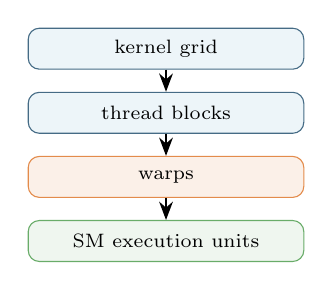
\begin{tikzpicture}[node distance=.28cm,every node/.style={font=\scriptsize},box/.style={draw=themebluedraw,fill=themebluebg,rounded corners,minimum width=3.5cm,minimum height=.52cm}]
        \node[box] (grid) {kernel grid};
        \node[box,below=of grid] (block) {thread blocks};
        \node[box,fill=warningbg,draw=warningdraw,below=of block] (warp) {warps};
        \node[box,fill=successbg,draw=successdraw,below=of warp] (sm) {SM execution units};
        \draw[-{Stealth},thick] (grid)--(block);
        \draw[-{Stealth},thick] (block)--(warp);
        \draw[-{Stealth},thick] (warp)--(sm);
      \end{tikzpicture}
    \end{column}
  \end{columns}
  \smallsource{JAX Scaling Book, How to Think About GPUs}
\end{frame}

\begin{frame}{Warps reward regular work}
  \begin{columns}[t]
    \begin{column}{0.47\linewidth}
      \begin{block}{Good utilization}
        contiguous access\\similar control flow\\enough active warps\\tile-aligned matrix dimensions
      \end{block}
    \end{column}
    \begin{column}{0.47\linewidth}
      \begin{alertblock}{Lost utilization}
        branch divergence\\strided loads\\register pressure\\tiny or awkward shapes
      \end{alertblock}
    \end{column}
  \end{columns}
  \vfill
  \centering A mathematically identical operation can run much faster when its layout and dimensions match the hardware tiles.
\end{frame}

\begin{frame}{The memory hierarchy trades capacity for speed}
  \centering\small
  \begin{tabular}{@{}>{\raggedright\arraybackslash}p{.22\linewidth}>{\raggedright\arraybackslash}p{.16\linewidth}>{\raggedright\arraybackslash}p{.13\linewidth}>{\raggedright\arraybackslash}p{.36\linewidth}@{}}
    \toprule
    Level & Scope & Capacity & Role \\
    \midrule
    registers & one thread & tiny & live scalar and fragment state \\
    shared memory / SRAM & one block or SM & small & explicit reuse and tiling \\
    L2 cache & whole device & moderate & cross-SM reuse \\
    HBM / VRAM & whole device & large & weights, activations, optimizer state \\
    host memory & CPU system & largest & dataset staging and overflow \\
    \bottomrule
  \end{tabular}
  \vfill
  \begin{alertblock}{Performance principle}
    Moving a value often costs more time and energy than performing one arithmetic operation on it. Reuse data near the compute units.
  \end{alertblock}
\end{frame}

\section{Roofline reasoning}

\begin{frame}{Arithmetic intensity predicts the limiting resource}
  \begin{columns}[c]
    \begin{column}{0.69\linewidth}
      \centering
      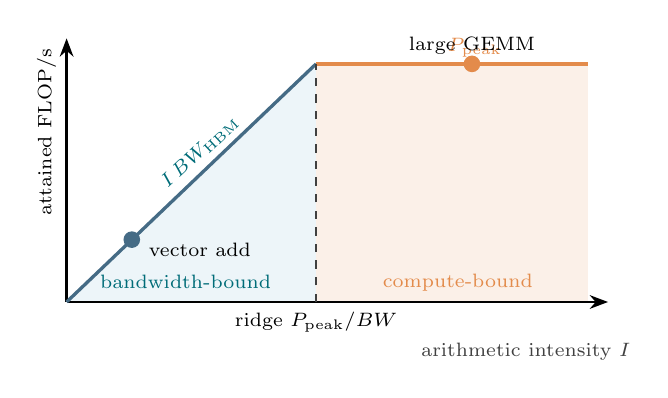
\begin{tikzpicture}[x=.72cm,y=.72cm,every node/.style={font=\scriptsize}]
        \fill[themebluebg] (0,0)--(4.4,4.2)--(4.4,0)--cycle;
        \fill[warningbg] (4.4,0)--(4.4,4.2)--(9.2,4.2)--(9.2,0)--cycle;
        \draw[-{Stealth},thick] (0,0)--(9.55,0);
        \draw[-{Stealth},thick] (0,0)--(0,4.65) node[above,rotate=90,anchor=south east]{attained FLOP/s};
        \draw[very thick,themebluedraw] (0,0)--(4.4,4.2);
        \draw[very thick,warningdraw] (4.4,4.2)--(9.2,4.2);
        \draw[dashed,neutraldark] (4.4,0)--(4.4,4.2);
        \node[rotate=43,text=accentdark] at (2.35,2.65) {$I\,BW_{\mathrm{HBM}}$};
        \node[text=warningdraw] at (7.2,4.48) {$P_{\mathrm{peak}}$};
        \fill[themebluedraw] (1.15,1.10) circle (3pt);
        \node[anchor=west] at (1.28,.92) {vector add};
        \fill[warningdraw] (7.15,4.2) circle (3pt);
        \node[above] at (7.15,4.2) {large GEMM};
        \node[below] at (4.4,0) {ridge $P_{\mathrm{peak}}/BW$};
        \node[below,text=neutraldark] at (8.1,-.55) {arithmetic intensity $I$};
        \node[text=accentdark] at (2.1,.35) {bandwidth-bound};
        \node[text=warningdraw] at (6.9,.35) {compute-bound};
      \end{tikzpicture}
    \end{column}
    \begin{column}{0.29\linewidth}
      \scriptsize
      \[
        I=\frac{F}{B_{\mathrm{HBM}}}
      \]
      \[
        P\le\min(P_{\mathrm{peak}},I\,BW)
      \]
      \begin{alertblock}{Read the lower roof}
        Moving right means reusing each loaded byte more.
      \end{alertblock}
    \end{column}
  \end{columns}
  \smallsource{JAX Scaling Book, How to Think About GPUs}
\end{frame}

\begin{frame}{Vector addition is memory-bound by construction}
  For $C=A+B$ with FP32 elements:
  \[
    \text{FLOPs}=1,\qquad \text{bytes}=4+4+4=12
  \]
  \[
    I\approx 0.083\ \text{FLOP/byte}
  \]
  \begin{block}{Prediction}
    Runtime scales with bytes moved. Kernel fusion can help by eliminating intermediate reads and writes.
  \end{block}
  \begin{alertblock}{Benchmark check}
    Doubling peak FLOPs should barely change runtime if memory bandwidth stays fixed.
  \end{alertblock}
\end{frame}

\begin{frame}{Large matrix multiplication creates reuse}
  For square $C=AB$, matrices of width $n$:
  \[
    \text{FLOPs}\approx2n^3,\qquad \text{minimum bytes}\approx3n^2s
  \]
  \[
    I\approx\frac{2n}{3s}
  \]
  Arithmetic intensity grows with $n$ because tiles of $A$ and $B$ are reused from SRAM.
  \begin{alertblock}{Small matrices behave differently}
    Launch overhead, poor tile occupancy, and insufficient reuse can keep small GEMMs far below peak compute.
  \end{alertblock}
\end{frame}

\begin{frame}{FlashAttention changes traffic, not the attention equation}
  Naive attention materializes the $T\times T$ score and probability matrices in HBM. FlashAttention tiles the computation and maintains online softmax statistics in SRAM.
  \begin{columns}[t]
    \begin{column}{0.47\linewidth}
      \begin{alertblock}{Naive path}
        write scores\\read for softmax\\write probabilities\\read to multiply values
      \end{alertblock}
    \end{column}
    \begin{column}{0.47\linewidth}
      \begin{block}{Tiled path}
        load $Q,K,V$ blocks\\update exact softmax statistics\\write only the final output
      \end{block}
    \end{column}
  \end{columns}
\end{frame}

\checkpoint{roofline diagnosis}
  {An optimization halves the FLOP count of a normalization kernel but runtime barely moves. Which roofline quantity explains the result, and what change is more promising?}

\section{Memory and measurement}

\begin{frame}{VRAM holds much more than model weights}
  \small
  \begin{tabular}{lll}
    \toprule
    Component & Typical scaling & Lifetime \\
    \midrule
    parameters & $P\times$ dtype bytes & whole run \\
    gradients & roughly $P$ & until update/reset \\
    Adam moments & roughly $2P$ in FP32 & whole run \\
    master weights & optional FP32 copy & whole run \\
    activations & $B,T,L,d$ dependent & forward to backward \\
    temporary buffers & kernel dependent & operation lifetime \\
    allocator reserve & fragmentation dependent & process lifetime \\
    \bottomrule
  \end{tabular}
  \vfill
  \begin{block}{Useful distinction}
    Report allocated and reserved memory. Out-of-memory behavior depends on peaks and fragmentation, not only steady-state tensor sizes.
  \end{block}
\end{frame}

\begin{frame}{Activation checkpointing exchanges compute for memory}
  \begin{columns}[c]
    \begin{column}{0.48\linewidth}
      \begin{alertblock}{Store everything}
        Faster backward pass\\higher activation memory\\larger feasible recomputation-free batch
      \end{alertblock}
    \end{column}
    \begin{column}{0.48\linewidth}
      \begin{block}{Checkpoint selected boundaries}
        Lower activation memory\\recompute forward segments in backward\\may enable larger $B$ or $T$
      \end{block}
    \end{column}
  \end{columns}
  \vfill
  Evaluate end-to-end tokens per second. A larger batch does not guarantee a faster run if recomputation dominates.
\end{frame}

\begin{frame}{Performance metrics answer different questions}
  \begin{columns}[t]
    \begin{column}{0.47\linewidth}
      \begin{block}{Throughput}
        tokens/s measures delivered training work\\step time exposes update cadence\\time-to-target includes optimization quality
      \end{block}
    \end{column}
    \begin{column}{0.47\linewidth}
      \begin{block}{Hardware efficiency}
        \[\mathrm{MFU}=\frac{\text{model FLOPs/s}}{\text{peak FLOPs/s}}\]
        MFU depends on the FLOP model and quoted peak precision.
      \end{block}
    \end{column}
  \end{columns}
\end{frame}

\begin{frame}{Read a profiler trace as a causal story}
  \begin{enumerate}
    \setlength{\itemsep}{7pt}
    \item Is the GPU idle between steps? Inspect input loading and synchronization.
    \item Are there many tiny kernels? Inspect fusion and compilation opportunities.
    \item Do copies overlap compute? Inspect pinned memory and asynchronous transfer.
    \item Does one kernel dominate? Classify it with shapes, bytes, and FLOPs.
    \item Are unexpected synchronizations present? Find scalar reads and host barriers.
  \end{enumerate}
\end{frame}

\begin{frame}{Apply optimizations in an evidence-driven order}
  \begin{enumerate}
    \setlength{\itemsep}{5pt}
    \item verify correctness and stabilize the benchmark
    \item keep the input pipeline ahead of the GPU
    \item use BF16 or FP16 safely
    \item select efficient scaled-dot-product attention
    \item fuse bandwidth-bound operation chains
    \item compile stable graphs and shapes
    \item checkpoint activations only when memory is the constraint
  \end{enumerate}
  \begin{alertblock}{One change per measurement}
    Warm up, synchronize, use enough repeated steps, and report median plus dispersion.
  \end{alertblock}
\end{frame}

\checkpoint{one-change ablation}
  {Choose one slow trace pattern. State the bottleneck hypothesis, the single intervention, the expected profiler change, and the correctness check that must remain unchanged.}

\takeaways
  {GPU speed comes from parallel regular work and data reuse, not from clock speed alone.}
  {Roofline reasoning separates bandwidth-bound from compute-bound operations.}
  {Peak memory includes activations, optimizer state, temporaries, and allocator behavior.}
  {A trustworthy speedup needs a stable workload, correctness checks, and causal profiling evidence.}

\end{document}
